\documentclass[11pt]{article}

\usepackage[preprint]{acl}

\usepackage{times}
\usepackage{latexsym}
\usepackage[T1]{fontenc}
\usepackage[utf8]{inputenc}
\usepackage{microtype}
\usepackage{inconsolata}
\usepackage{graphicx}
\usepackage{booktabs}
\usepackage{multirow}
\usepackage{subcaption}
\usepackage{url}

\title{DeafConnect: A Mobile System for American Sign Language Recognition\\and Bidirectional Translation}

\author{Elie Shakkour \and Jad Antoun \\
  \textit{Supervisor: Dr Chadi Helwe} \\[0.3em]
  \small Code: \url{https://github.com/jadantoun9/deafconnect} \\}

\begin{document}
\maketitle

\begin{abstract}
Sign language recognition on a mobile phone is two problems at once. The first is statistical: most published models on benchmarks such as WLASL are trained and evaluated offline on a GPU, with no constraint on latency, model size or supported operations. The second is engineering: a deployable assistive tool has to run on the device the user already owns, in real time, in both directions (sign-to-text and text-to-sign), and without uploading the camera feed to a remote server. This paper presents \textbf{DeafConnect}, an iOS system that addresses both problems jointly. The system contains two recognition tracks: a feed-forward classifier over MediaPipe hand landmarks for the 26 letters of the American Sign Language alphabet, and a Transformer over MediaPipe Holistic landmarks for word-level signs. Both are exported to Apple's CoreML format and run on the Apple Neural Engine. The deployed letter model reaches \textbf{93.32\%} accuracy on a held-out 1{,}302-sample test set. For words, pruning the Holistic skeleton from 75 to 48 keypoints lifts validation top-1 accuracy from 65.0\% to 80.0\% on a 9-class WLASL subset, and the same model beats a frozen ViT-S/16 video baseline by 28 absolute points on the six sign classes both can predict. The application also includes a chat tab that uses on-device speech-to-text and text-to-speech, and a text-to-sign tab driven by a Ready Player Me 3D avatar. Source code, configs, training scripts and the iOS application are released.
\end{abstract}

\section{Introduction}

The World Federation of the Deaf estimates that more than 70 million people use a sign language as their primary mode of communication, with at least 200 distinct sign languages in active use across the world. American Sign Language (ASL) is the dominant sign language in the United States and parts of Canada. Day-to-day communication between deaf signers and the hearing population is overwhelmingly mediated by professional interpreters --- expensive, scheduled in advance, and unavailable in spontaneous settings --- or by handwriting, which is slow and disrupts the flow of conversation. A practical assistive tool for everyday use needs to fit on the device the user already owns and translate, in both directions, in real time.

The research literature has so far addressed only part of this problem. Word-level video classifiers such as Pose-TGCN and I3D \citep{li2020wlasl, carreira2017quo} report strong offline accuracy on the WLASL benchmark, but the models are large and the inference pipelines GPU-bound; almost none of the published systems are accompanied by an on-device latency budget on a phone. Alphabet-level classifiers on the Kaggle ASL Alphabet dataset are well studied as a teaching benchmark, but they recognise individual fingerspelled letters rather than full signs and rarely report cross-signer generalisation. The translation direction --- from typed or spoken text back into a sign-language output that the deaf user can follow --- is almost always omitted entirely. There is no published system, to our knowledge, that combines all three on a single phone.

\textbf{Contributions.} This work bridges that gap. The system, called \emph{DeafConnect}, is a complete end-to-end mobile pipeline that we release as open source. The technical contributions of the paper are the following.

\begin{enumerate}
\itemsep -0.1em
\item A \textbf{two-track recognition architecture} that uses a lightweight feed-forward classifier on hand landmarks for the 26-letter ASL alphabet and a small Transformer on body-and-hand landmarks for a working vocabulary of word-level signs. The two tracks share a common MediaPipe front-end and a common iOS application shell.
\item A controlled comparison of four alphabet classifiers, with a discussion of how dataset shortcuts in the standard Kaggle benchmark lead the image-based model to overstate its true generalisation.
\item A \textbf{keypoint-pruning ablation} on a 9-class subset of WLASL, showing that dropping head and lower-body landmarks from the MediaPipe Holistic skeleton (reducing the input from 75 to 48 keypoints) lifts validation top-1 accuracy from 65.0\% to 80.0\% with the same architecture and schedule.
\item A working \textbf{CoreML deployment} on iPhone. All four word-level models and the alphabet model are exported to \texttt{.mlpackage} and run on the Apple Neural Engine at 30\,fps, with no server round-trip.
\item A complete \textbf{bidirectional user-facing application} that wraps the recognition models in a chat experience using on-device speech-to-text and text-to-speech, and a text-to-sign tab driven by a Ready Player Me 3D avatar.
\end{enumerate}

Our aim is not to push state-of-the-art accuracy on WLASL: the WLASL test partitions are too small to make that claim at our scale. Our aim is to characterise what kind of accuracy is achievable when the modelling and deployment choices are jointly constrained to those that fit on a phone, and to ship the result as a usable product.

\section{Related Work}

\paragraph{Word-level recognition.} \citet{li2020wlasl} released WLASL, the standard benchmark for isolated word-level ASL recognition. They reported I3D \citep{carreira2017quo} and Pose-TGCN baselines, with I3D reaching about 32\% top-1 on the full 2000-class vocabulary. Later work has tried skeleton transformers, self-supervised pretraining and multi-modal fusion. Most of these models are large and assume a GPU at inference time.

\paragraph{Alphabet recognition.} The Kaggle ASL Alphabet dataset \citep{aslalphabet2018} is widely used as a teaching benchmark. Most public solutions get above 95\% on it. The dataset has a known weakness: all images were collected in one session, so a random train/test split leaks signer, lighting and background. A model can score very high on test and still fail in the real world. We see this directly in our own results.

\paragraph{Landmark extraction.} MediaPipe Hands and MediaPipe Holistic \citep{lugaresi2019mediapipe, zhang2020mediapipe} give real-time hand and body landmarks on a phone. The hand model returns 21 keypoints. The Holistic pipeline adds 33 body pose keypoints. Both run on iOS, which is what we needed.

\paragraph{Vision transformers and token merging.} The Vision Transformer \citep{dosovitskiy2021an} is now the default image backbone. For video, the usual recipe is to apply a frozen image ViT per frame and add a small temporal head on top. Token Merging \citep{bolya2023token} reduces the inference cost of ViT by merging similar tokens. We use a frozen ViT-S/16 with a 3-layer temporal Transformer as our Track 2 baseline.

\paragraph{On-device ML for accessibility.} Practical on-device sign-language tools are rare. Most apps either send frames to a server or only handle the alphabet. CoreML and the Apple Neural Engine give us very fast inference, but only if the model uses ops on a restricted list. That constraint shaped some of our design choices.

\section{Datasets}

We use two public datasets.

\subsection{ASL Alphabet}

The Kaggle ASL Alphabet dataset has roughly 500 RGB images per letter for the 26 letters of the fingerspelled alphabet. We resize images to $64\times64$ for the image-based models. For the landmark-based models we run MediaPipe Hands on the original frame and store the resulting $21\times3$ tensor. Frames where MediaPipe failed to find a hand are dropped from the landmark dataset. We split 70/15/15 train/val/test with a fixed seed. Table~\ref{tab:asl-alphabet-splits} shows the final sizes.

\begin{table}[t]
\centering
\small
\begin{tabular}{lrrr}
\toprule
Modality & Train & Val & Test \\
\midrule
Landmarks ($21\times3$) & 6{,}071 & 1{,}301 & 1{,}302 \\
Images ($64\times64\times3$) & 9{,}099 & 1{,}951 & 1{,}950 \\
\bottomrule
\end{tabular}
\caption{ASL Alphabet split sizes. The landmark split is smaller because we drop frames where no hand is detected.}
\label{tab:asl-alphabet-splits}
\end{table}

\subsection{WLASL Subsets}

WLASL \citep{li2020wlasl} is the standard benchmark for isolated word-level ASL. It has roughly 21{,}000 clips across 2{,}000 signs. The usual research subsets are WLASL-100, 300, 1000 and 2000. We work with three configurations.

\textbf{WLASL-100} (100 classes, $\sim$600 clips, 409 / 115 / 76 train/val/test) is the standard benchmark used to give a comparable number against the literature.

\textbf{WLASL-9idle} (9 classes, 125 clips, 92 / 20 / 13) combines eight everyday signs --- \textit{drink, go, help, who, yes, no, before, walk} --- with an extra \textit{idle} class. We use this for the deployed Track 1 model. The idle class matters because the phone is always looking at the user; without it the model would predict a random sign whenever the user is just sitting there.

\textbf{WLASL-9} (8 classes, no idle, 108 clips, 80 / 17 / 11) is used for the end-to-end video baseline.

For Track 1 we precompute MediaPipe Holistic landmarks and cache them as $75\times3$ tensors per frame. For Track 2 we keep the resized $224\times224$ frames. Both test sets are very small, which we come back to in the discussion.

\section{Approach}

DeafConnect has two recognition tracks and one app that ties them together. Figure~\ref{fig:app} shows the two recognition modes running live.

\begin{figure*}[t]
\centering
\begin{subfigure}{0.24\textwidth}
  \centering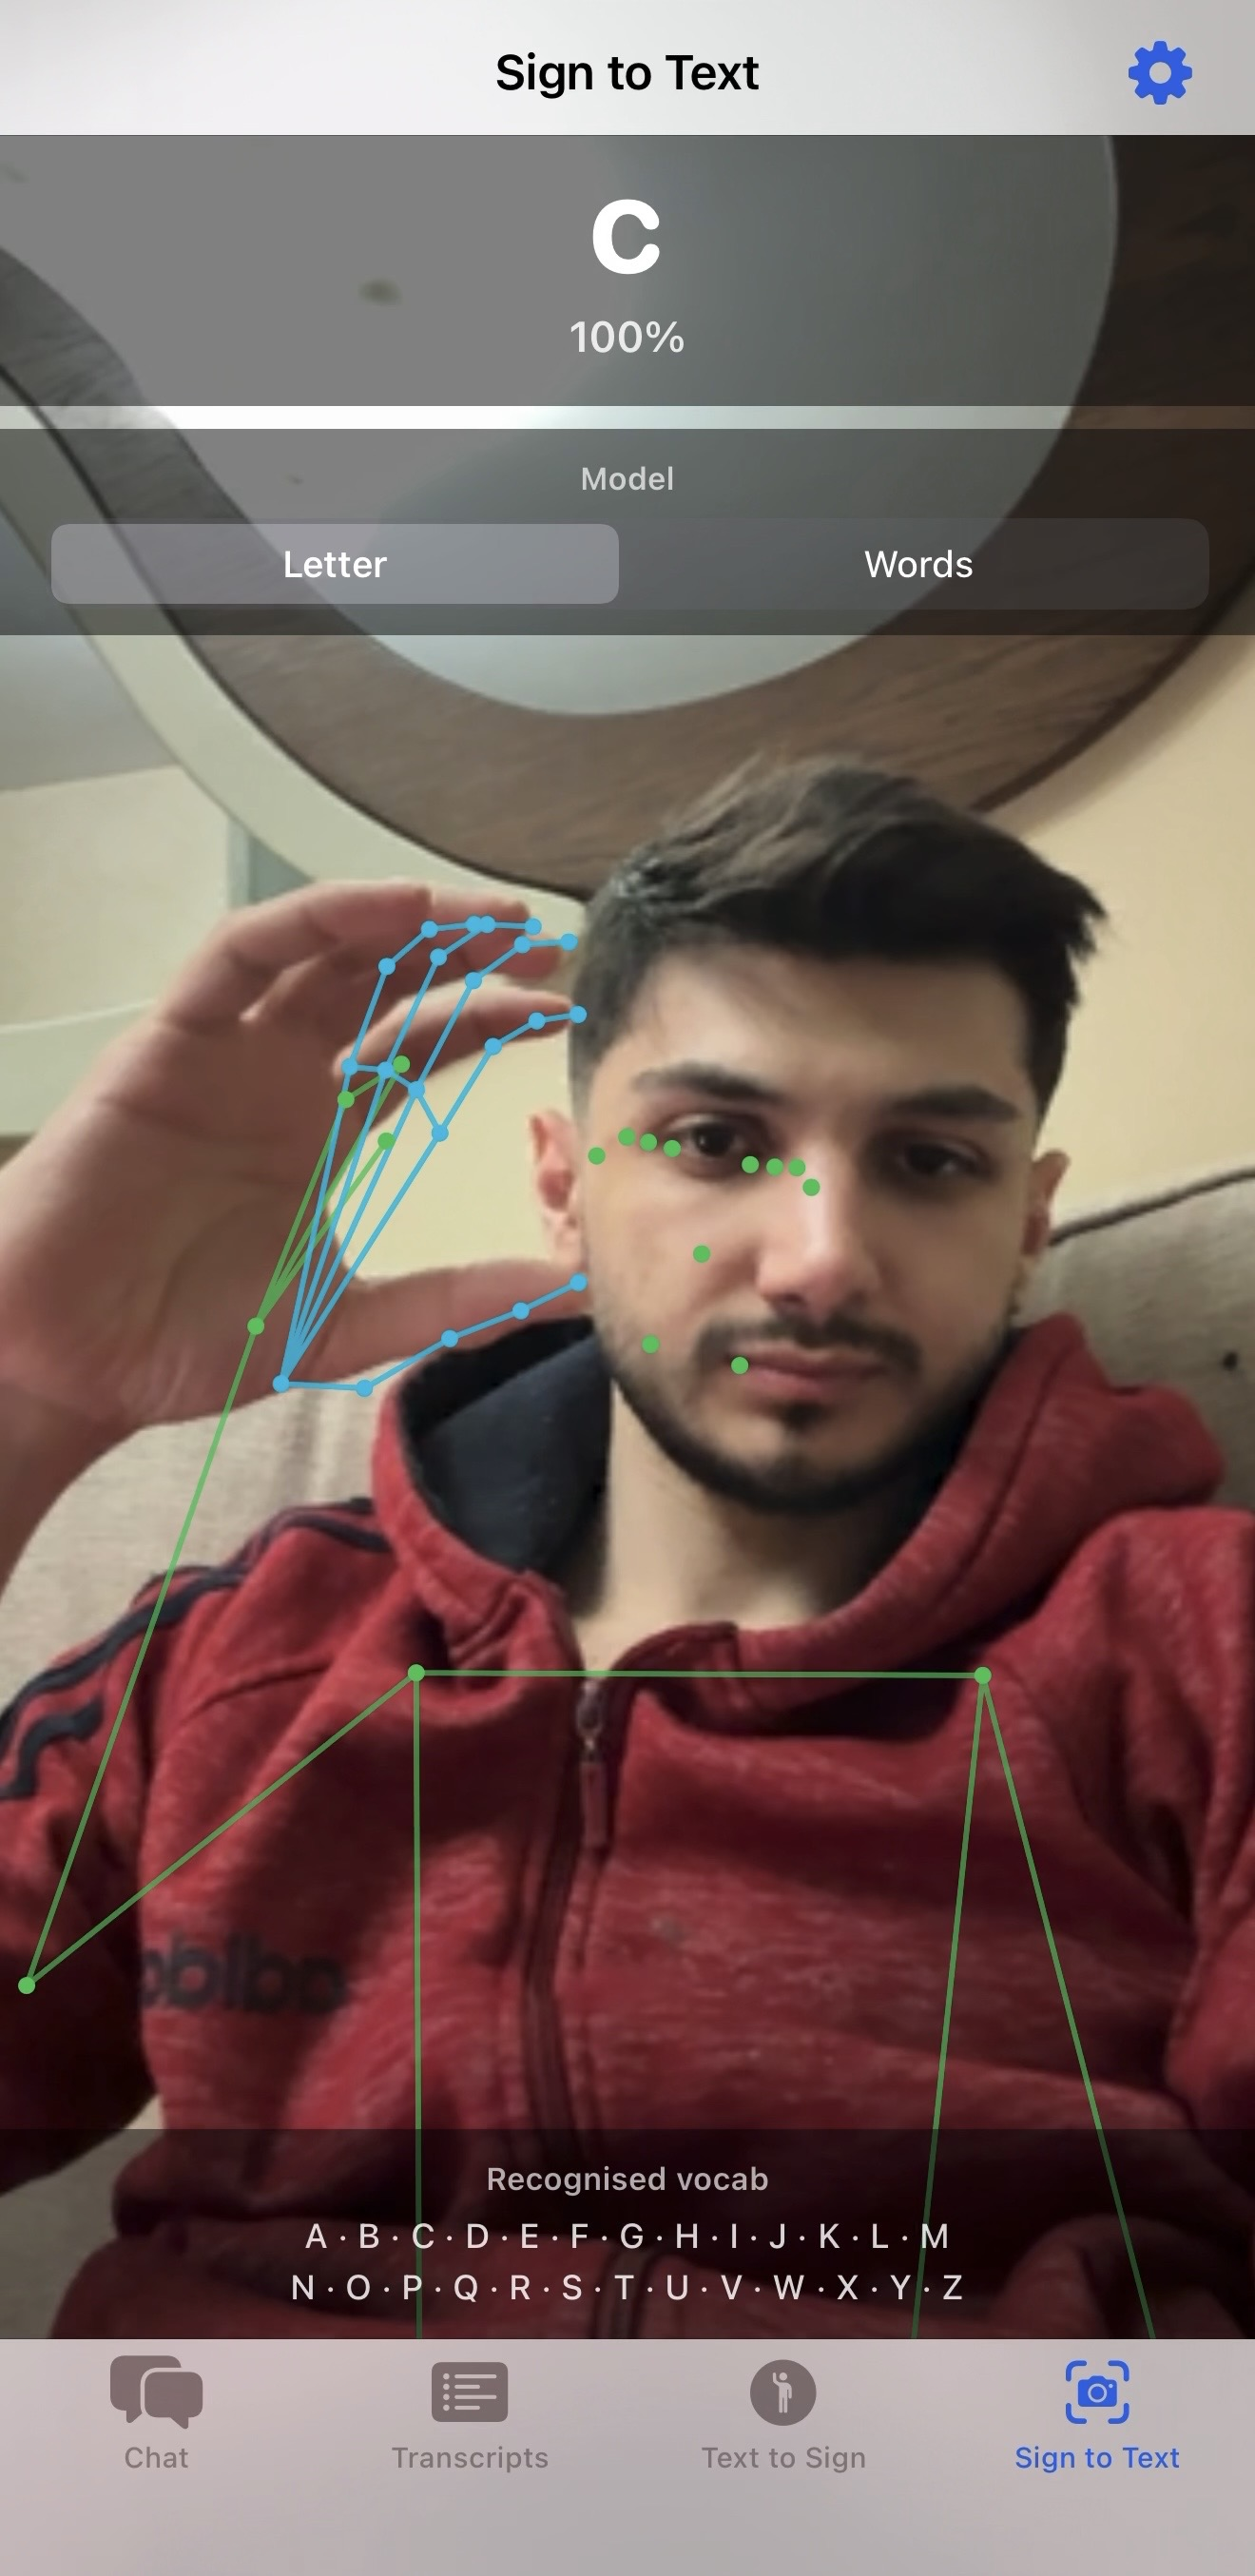
\includegraphics[width=\linewidth]{../app-images/sign-c.jpg}
  \caption{Letter \emph{C} (100\%)}
\end{subfigure}\hfill
\begin{subfigure}{0.24\textwidth}
  \centering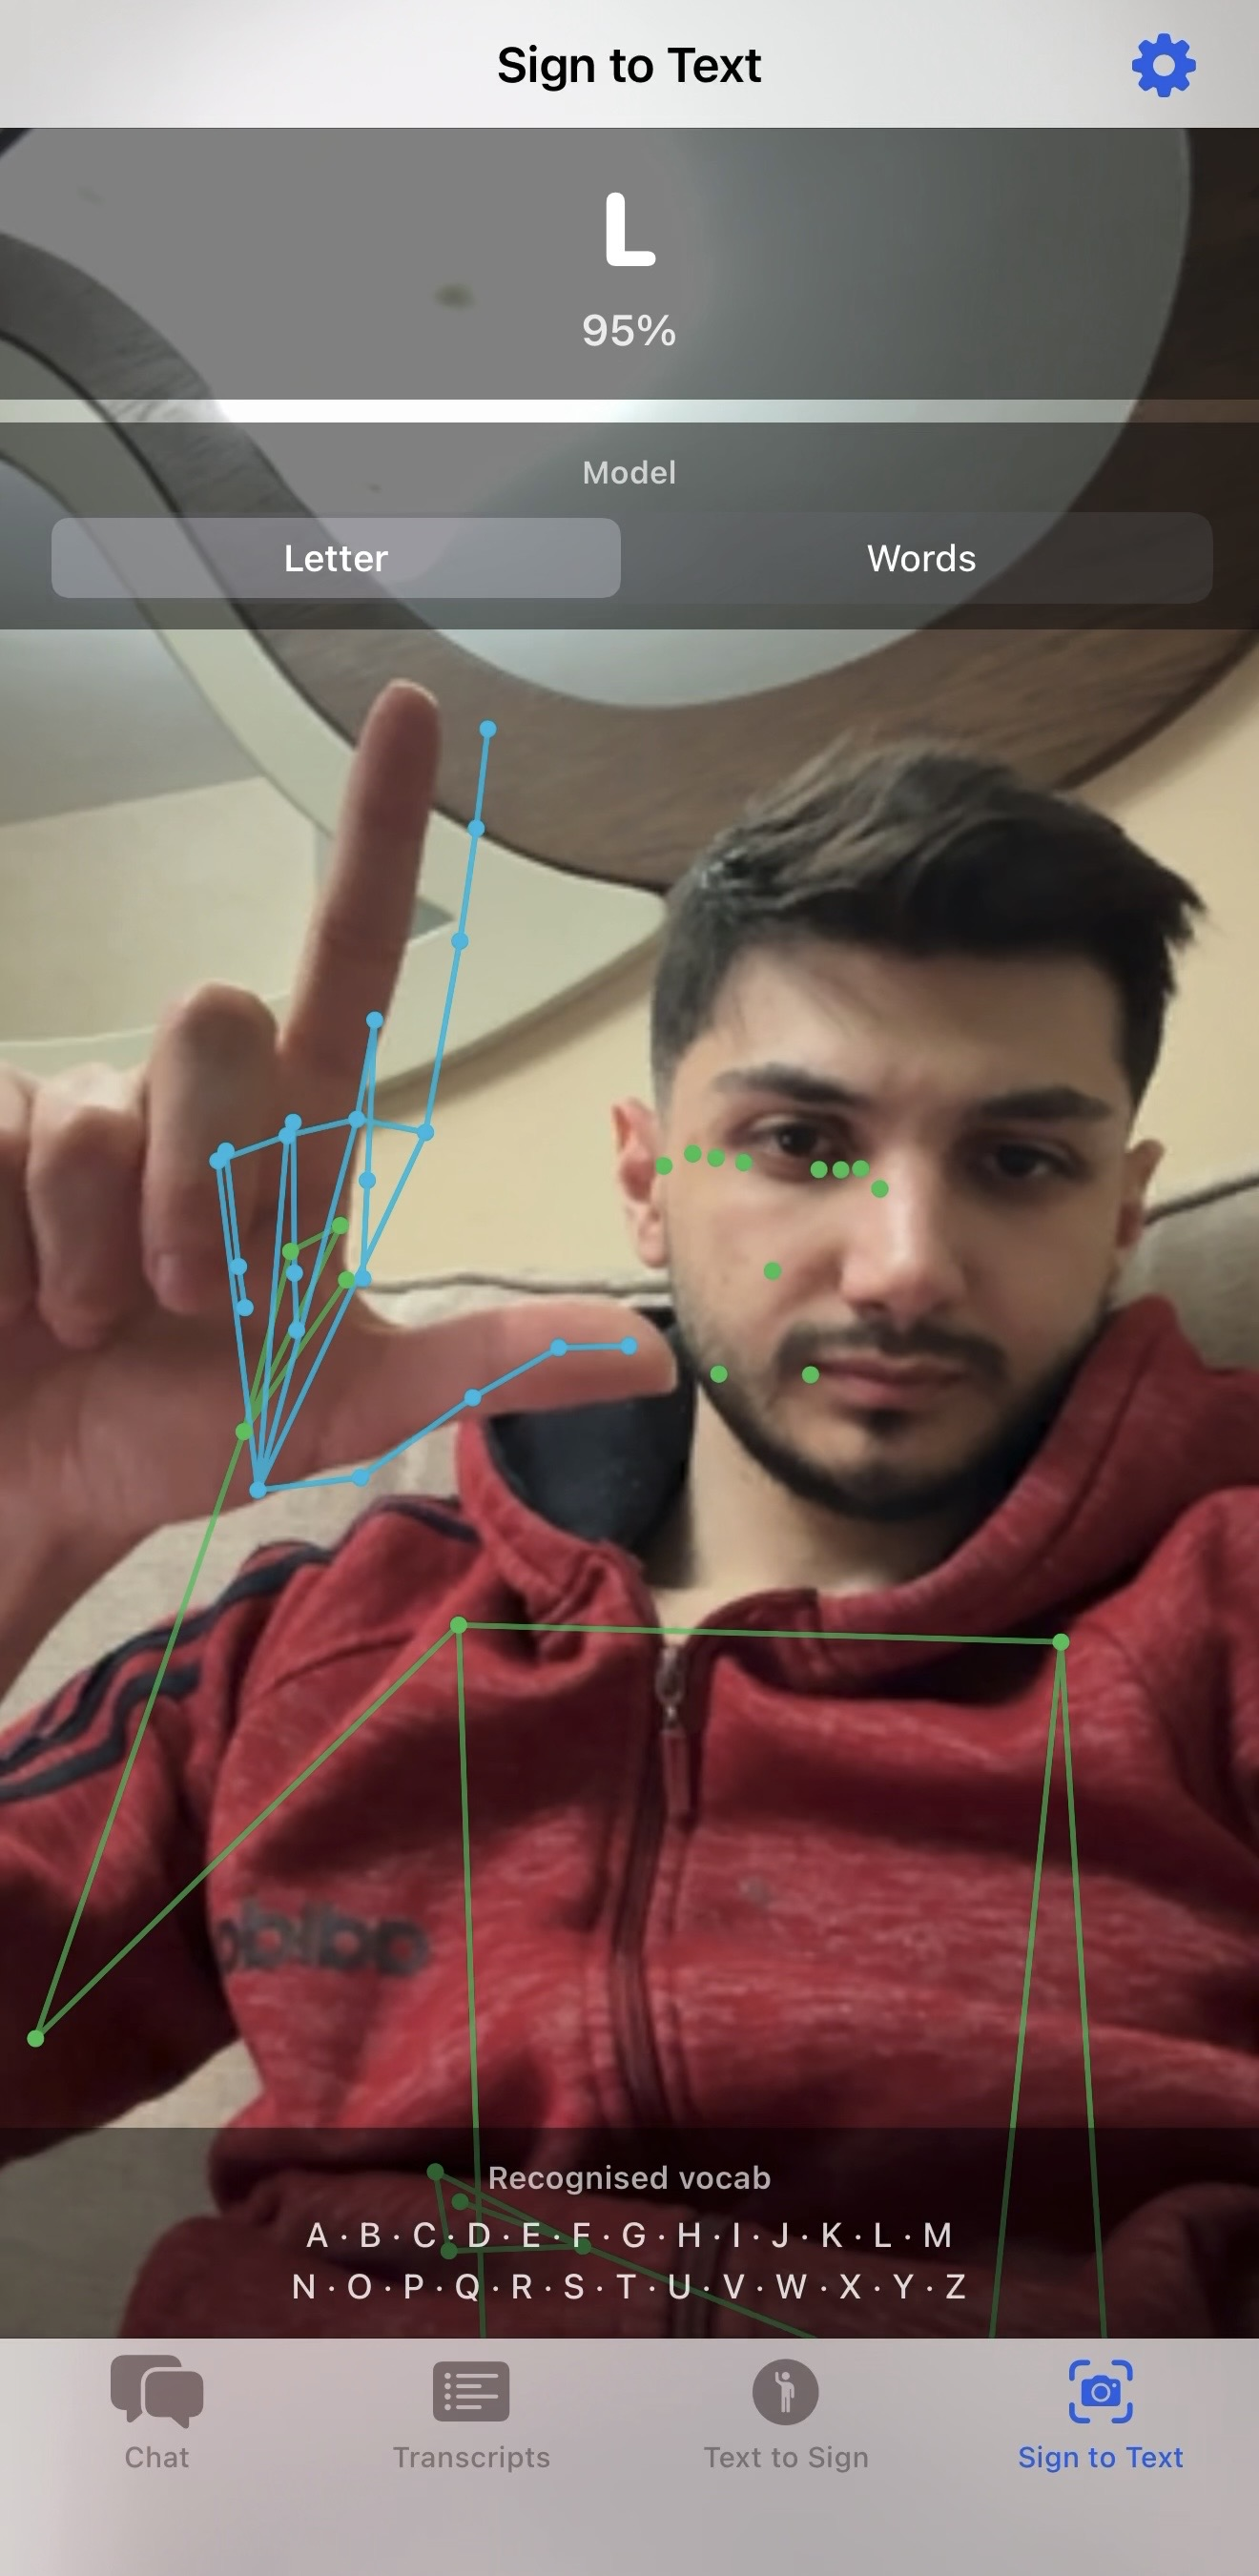
\includegraphics[width=\linewidth]{../app-images/sign-l.jpg}
  \caption{Letter \emph{L} (95\%)}
\end{subfigure}\hfill
\begin{subfigure}{0.24\textwidth}
  \centering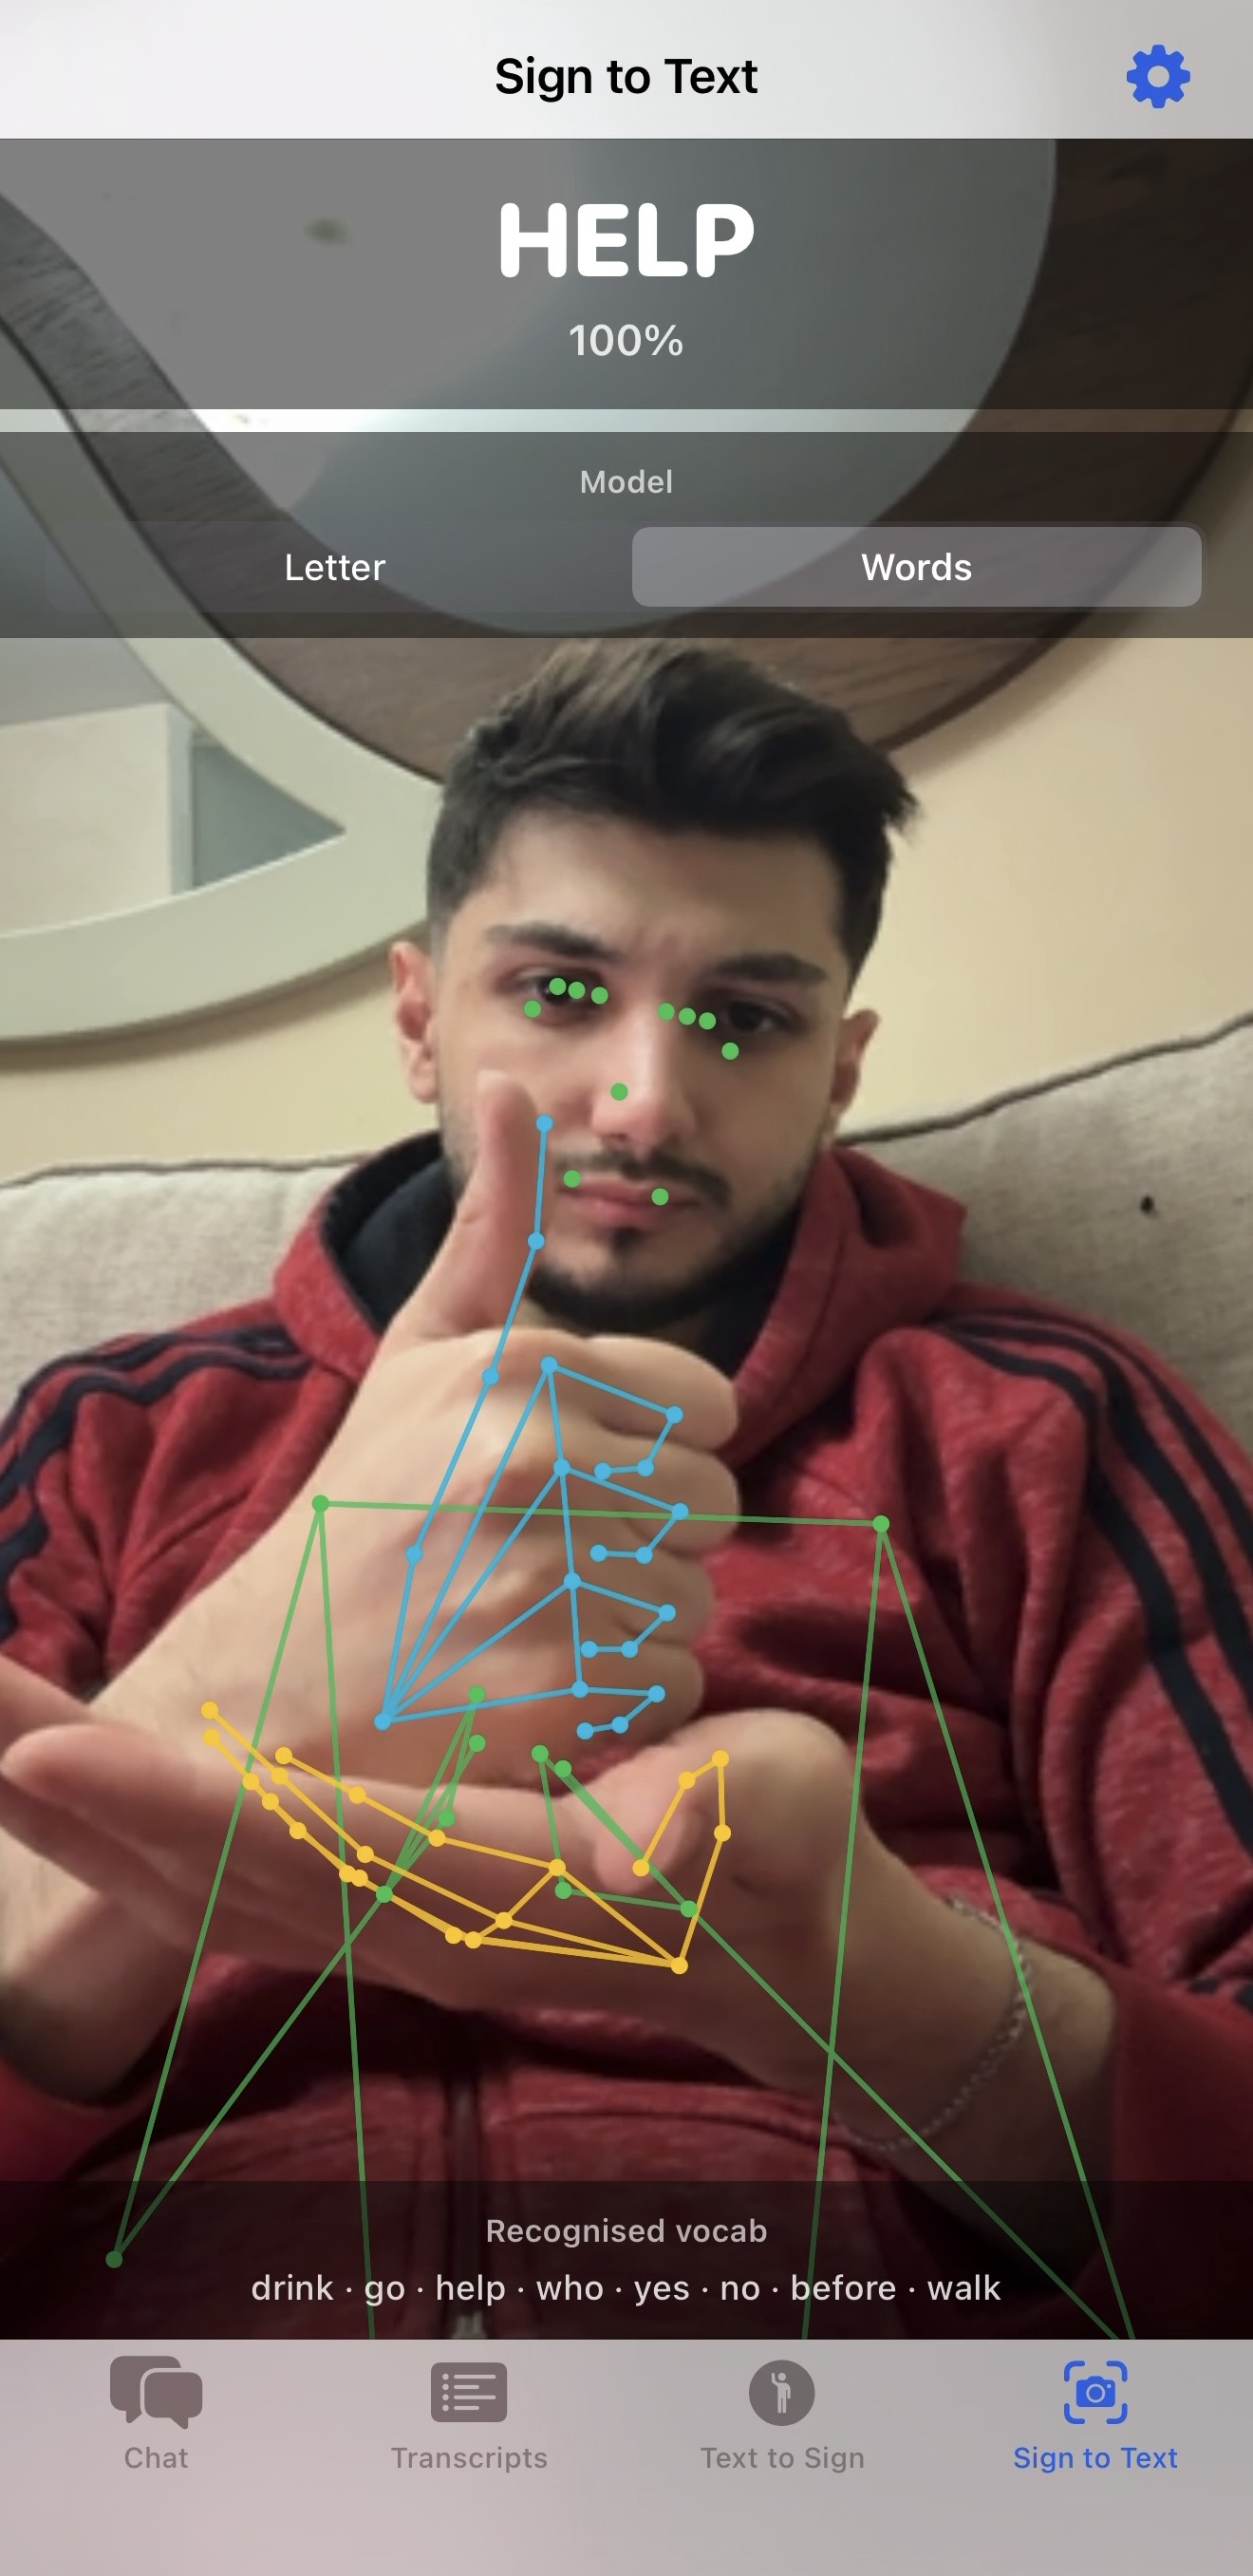
\includegraphics[width=\linewidth]{../app-images/sign-help.jpg}
  \caption{Word \emph{HELP} (100\%)}
\end{subfigure}\hfill
\begin{subfigure}{0.24\textwidth}
  \centering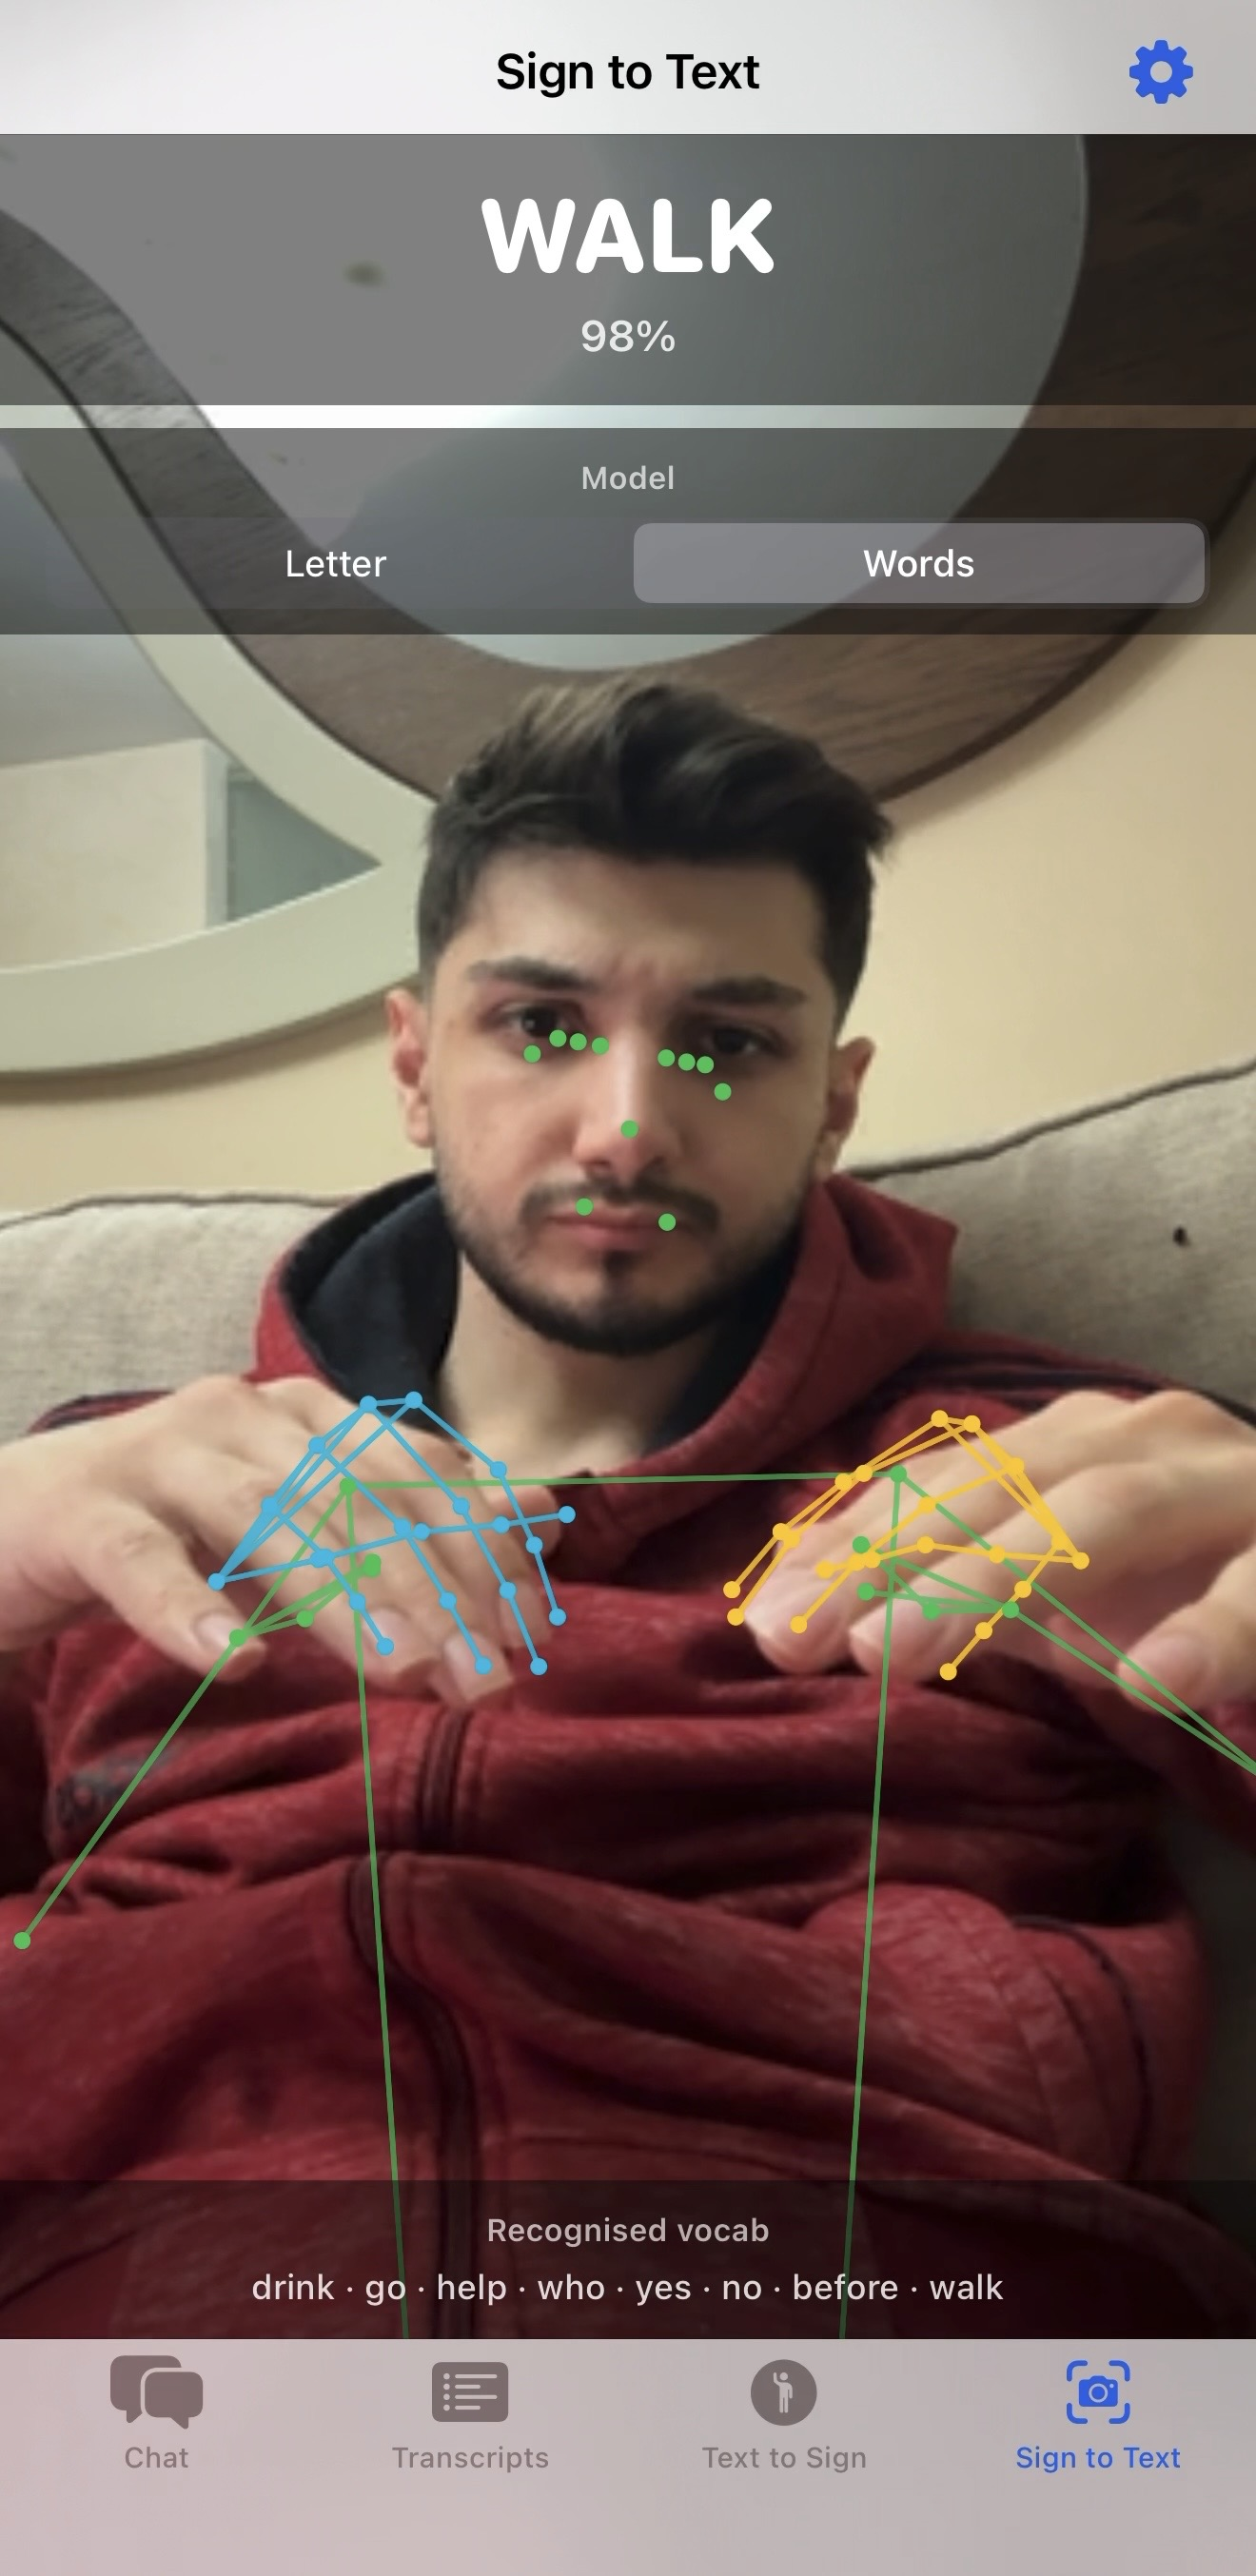
\includegraphics[width=\linewidth]{../app-images/sign-walk.jpg}
  \caption{Word \emph{WALK} (98\%)}
\end{subfigure}
\caption{The Sign-to-Text tab running on an iPhone. Letters (left) are read from 21 hand landmarks on a single frame. Words (right) are read from a 32-frame window of body and hand landmarks. The MediaPipe overlay shows the keypoints used by the model.}
\label{fig:app}
\end{figure*}

\subsection{Track 1 --- Landmark Models}

Both the letter model and the word model take MediaPipe landmarks as input. Landmarks have three nice properties for a phone app: they are cheap to compute, they ignore background and lighting, and they are robust to skin tone because the MediaPipe detector was trained on a broad set of users.

\paragraph{Letter model.} We tried four architectures and kept the best one. The deployed model is a feed-forward network with the shape \texttt{Flatten($63$) $\rightarrow$ Dense$_{512}$ $\rightarrow$ ReLU $\rightarrow$ Dense$_{256}$ $\rightarrow$ ReLU $\rightarrow$ Dense$_{26}$}. After Bayesian tuning over learning rate, hidden sizes and batch size, this model reaches 93.32\% test accuracy.

\paragraph{Word model.} For the 9-class word model we use a 2-layer Transformer encoder with $d_{\textrm{model}}=128$, 4 heads, feed-forward dimension 256, GELU activations and pre-norm. The input is a $[T\times K\times 3]$ tensor with $T=32$ frames and $K$ keypoints. Each frame is linearly projected to $d_{\textrm{model}}$ and added to a learnable positional embedding. The Transformer output is mean-pooled across valid frames (using MediaPipe's per-keypoint validity mask as a weight) and projected to the class logits. Total parameter count is about 150K.

We designed the model so that every operation in the forward pass lives on the Apple Neural Engine. That means no \texttt{nn.Embedding} (we replace it with a broadcasted \texttt{nn.Parameter}), no dynamic-shape ops, and only activations from the supported list (GELU, softmax, layer norm).

\subsection{Keypoint Pruning}

The MediaPipe Holistic pipeline returns 33 body pose keypoints, 21 keypoints per hand, and a 468-point face mesh. We turn off the face mesh during extraction, leaving 75 keypoints. For the V2 variant of the word model we further drop:

\begin{itemize}
\itemsep -0.1em
\item 11 head keypoints (nose, eyes, ears, mouth corners);
\item 2 hip keypoints;
\item 8 lower-body keypoints (knees, ankles, heels, feet);
\item 6 coarse hand landmarks that the pose model returns but which are already covered by the dedicated hand mesh.
\end{itemize}

That leaves 48 keypoints: six upper-body anchors (shoulders, elbows, wrists) plus the two 21-point hand meshes. The idea is simple. Head and leg keypoints move on their own, independent of the sign --- the signer may tilt the head or shift weight --- and the model has to learn to ignore them. Removing them up front saves capacity and reduces input noise.

\subsection{Track 2 --- Video Model}

Track 2 is a frozen ViT-S/16 backbone with a small temporal head, the standard recipe for video classification when training data is limited. We load \texttt{vit\_small\_patch16\_224.augreg\_in21k\_ft\_in1k} from \texttt{timm} and freeze it. Each frame becomes $14\times14=196$ patch tokens of dimension 384. On top we add a 3-layer Transformer ($d_{\textrm{model}}=384$, 6 heads, feed-forward 768, dropout 0.2). The temporal head adds a learnable positional embedding along the time axis. The whole stack runs over $T=16$ frames.

\subsection{Comparison Across Tracks}

\begin{figure}[t]
\centering
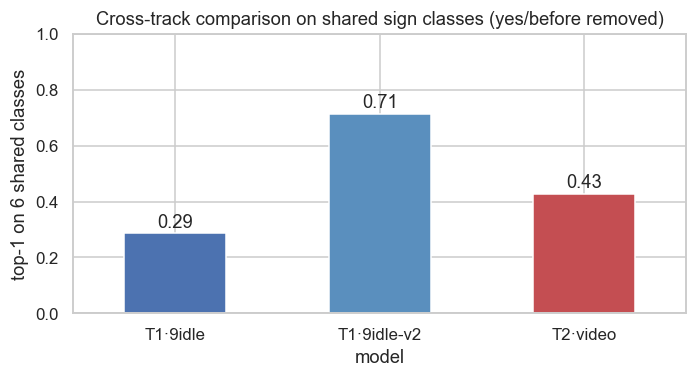
\includegraphics[width=0.95\linewidth]{../word-results/output88.png}
\caption{Headline comparison of the three word-level configurations on the six sign classes shared between Track 1 and Track 2 (\textit{drink, go, help, who, no, walk}). The pruned 48-keypoint landmark model (T1$\cdot$9idle-v2) reaches 0.71 top-1, against 0.43 for the frozen ViT-S/16 video baseline (T2$\cdot$video) and 0.29 for the full 75-keypoint landmark model (T1$\cdot$9idle). At the data scale available in WLASL-9, a 150K-parameter Transformer on a hand-engineered keypoint subset outperforms a 123\,MB ViT-based video backbone by a wide margin.}
\label{fig:cross}
\end{figure}

Before turning to the deployment and experimental details, Figure~\ref{fig:cross} previews how the three word-level configurations compare on the same six-class evaluation. The ranking holds throughout the rest of the paper: the pruned 48-keypoint landmark model is the strongest, the full 75-keypoint version is the weakest, and the end-to-end ViT video model lands in between. This ordering is what motivates the keypoint-pruning ablation in Section~\ref{sec:experiments} and the choice of the V2 model as the deployed recognition path on the phone.

\subsection{Mobile Deployment with CoreML}

\begin{table}[t]
\centering
\small
\begin{tabular}{lrl}
\toprule
Model & Size & Input shape \\
\midrule
Letter (26 classes)      & $\sim$5\,MB  & $[1, 21, 3]$ \\
Words V1 (9 cls, 75 kp) & 3.6\,MB & $[1, 32, 75, 3]$ \\
Words V2 (9 cls, 48 kp) & 3.4\,MB & $[1, 32, 48, 3]$ \\
Video (8 classes)        & 123.5\,MB & $[1, 16, 3, 224, 224]$ \\
\bottomrule
\end{tabular}
\caption{Deployed CoreML model sizes and input shapes. All four models live inside the same app and can be switched at runtime.}
\label{tab:coreml}
\end{table}

The trained PyTorch and Keras models are exported to Apple's \textbf{CoreML} format (\texttt{.mlpackage}) using \texttt{coremltools}. For the PyTorch models we go through ONNX (opset 17). We use fp16 weights and fixed input shapes (no dynamic axes) so the CoreML compiler can place the whole graph on the Apple Neural Engine. The result is in Table~\ref{tab:coreml}.

Running on the Neural Engine is what makes the app work in real time. Letter and landmark word models run in well under 10\,ms per inference. The video model is much heavier but still keeps up at 30\,fps because we only feed it 16 frames. Just as important, nothing leaves the phone. There is no server. The user's camera feed is never uploaded. This matters for accessibility tools, where the camera is pointed at the user's face all day and any cloud round-trip is both a privacy issue and a latency issue.

\subsection{The Mobile App}

The app, called \emph{SignReader}, has four tabs. We describe them in the order a typical user would meet them.

\paragraph{Chat.} The main tab is a real-time chat for deaf users (Figure~\ref{fig:bidir}, left). It looks like a normal messaging screen with two parties. The deaf user types or signs a message. The hearing partner speaks into the phone, and the app uses iOS speech-to-text to turn their voice into a written reply. The deaf user can tap a speaker icon next to any message and the app reads it out with text-to-speech, so the partner does not need to read the screen. The whole exchange becomes a normal-looking conversation. This is where the app spends most of its time in practice --- ordering at a restaurant, asking for help in a shop, talking to a doctor.

\paragraph{Transcripts.} Past chats are saved as transcripts. A user can open the history, scroll a conversation and replay any line. This is useful for follow-ups (``what did the doctor say about the prescription?'') and for sharing context with family.

\paragraph{Text-to-Sign.} The third tab takes typed or spoken text and plays it back as ASL using a 3D animated avatar (Figure~\ref{fig:bidir}, right). The avatar is built with Ready Player Me. Two roles for this tab. First, a deaf user can show a hearing partner an example sign they want to learn. Second, and more important, a hearing user who is starting to learn ASL can use the avatar as a personal tutor: they type a word and watch the avatar perform it from several angles. The current avatar fingerspells the input. A learned sign-synthesis model is a natural extension and is left as future work.

\paragraph{Sign-to-Text.} The fourth tab is what the recognition models drive. The user points the phone's front camera at themselves, picks Letter or Word mode, and the predicted label appears at the top of the screen along with the model's confidence (Figure~\ref{fig:app}). The MediaPipe landmark overlay shows what the model is looking at. The main audience here is the hearing partner: they want to understand what the deaf user is signing, in cases where the partner has no ASL background.

\begin{figure}[t]
\centering
\begin{subfigure}{0.46\linewidth}
  \centering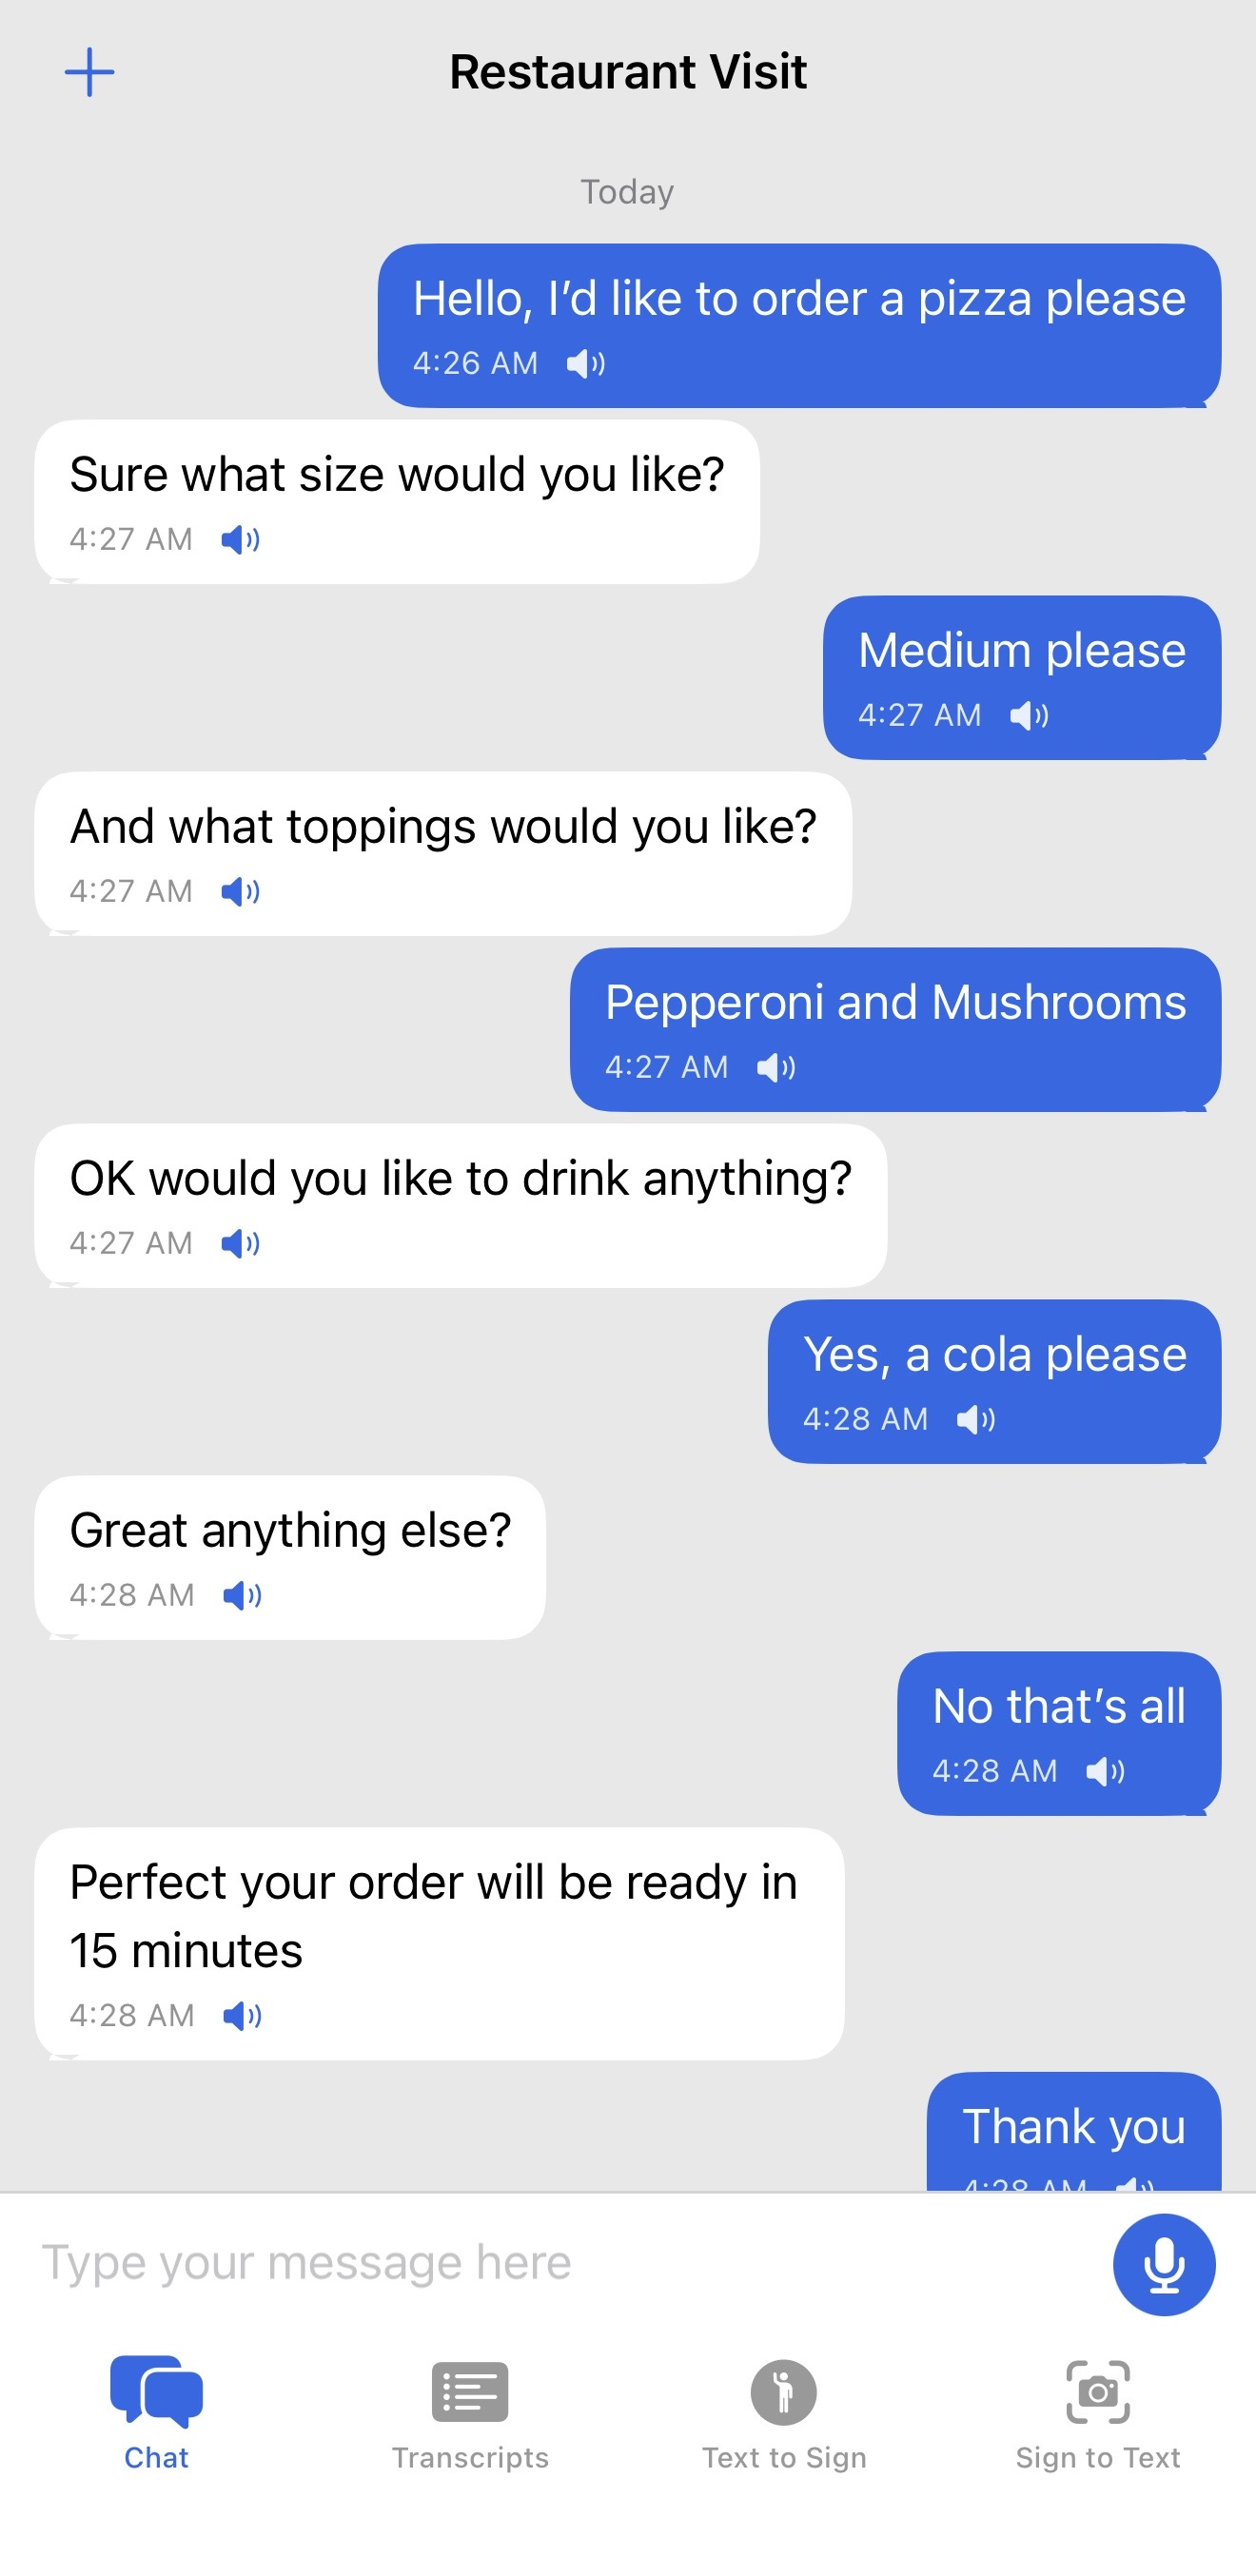
\includegraphics[width=\linewidth]{../app-images/chat.jpg}
  \caption{Chat tab}
\end{subfigure}\hfill
\begin{subfigure}{0.46\linewidth}
  \centering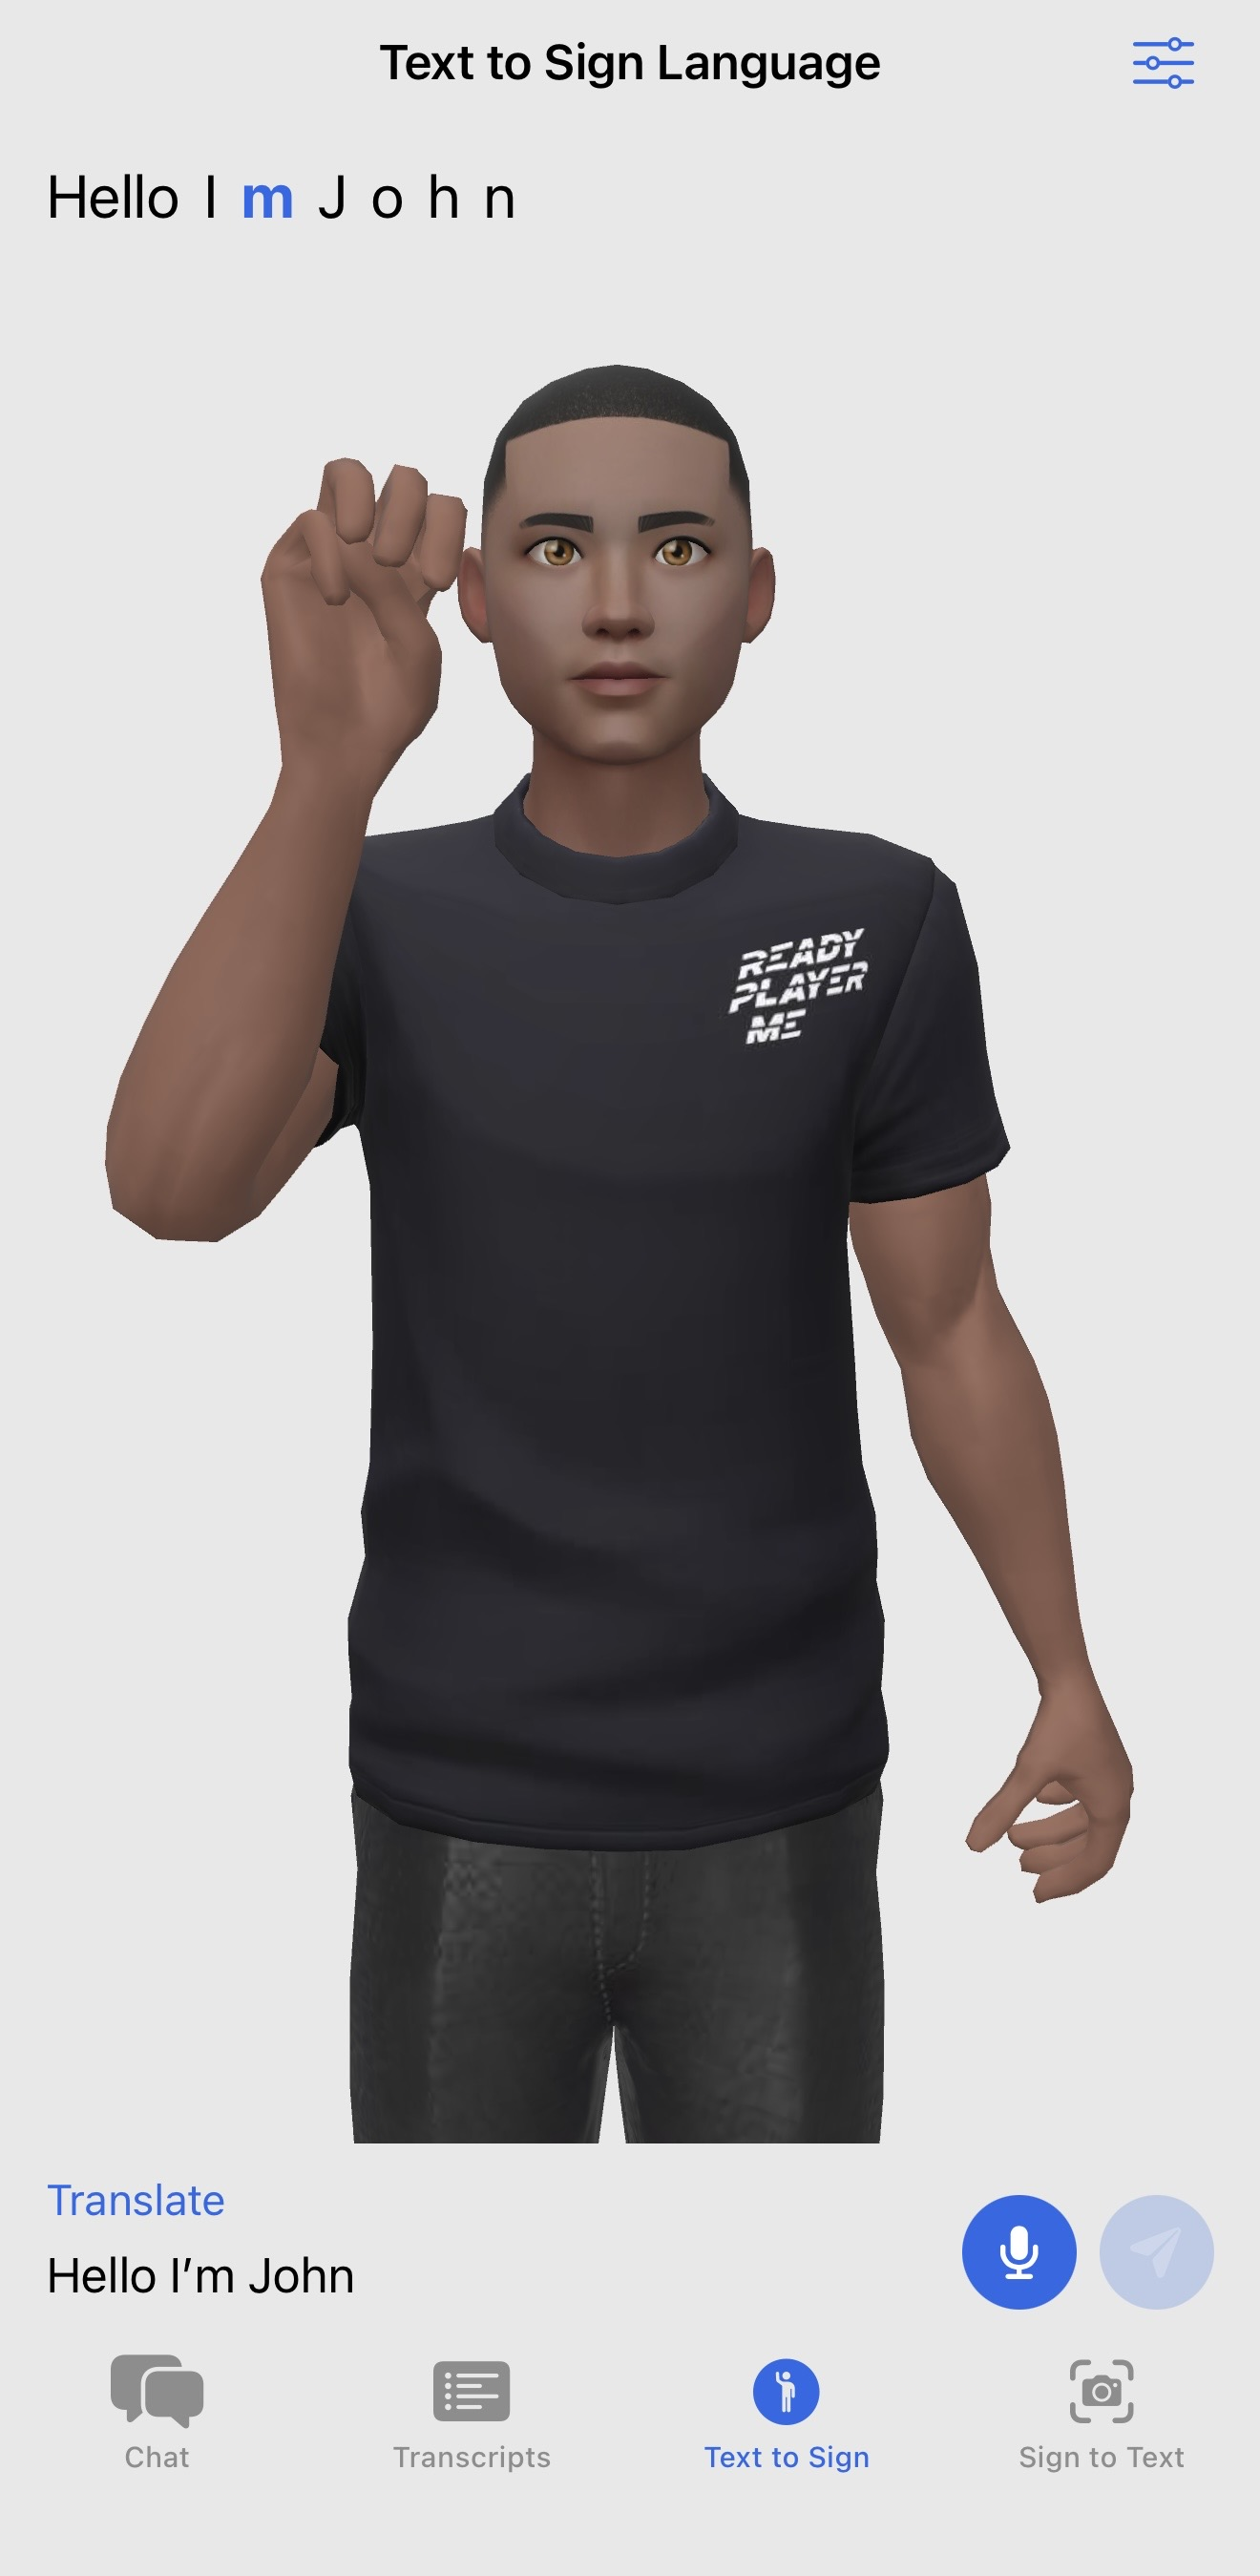
\includegraphics[width=\linewidth]{../app-images/avatar-m.jpg}
  \caption{Text-to-Sign avatar}
\end{subfigure}
\caption{Left: the Chat tab. The deaf user has a normal-looking conversation thread with a hearing partner. A speaker icon next to each message plays text-to-speech; a microphone button captures the partner's voice via on-device speech-to-text. Right: the Text-to-Sign tab. A Ready Player Me avatar plays the input sentence in ASL, letter by letter. Useful as a personal tutor for hearing users learning ASL.}
\label{fig:bidir}
\end{figure}

\section{Experiments}\label{sec:experiments}

\subsection{Training Setup}

\paragraph{ASL Alphabet.} The four letter models are trained with Adam, learning rate $10^{-3}$, batch size 32, 10 epochs. We keep the 15\% test split for final reporting and use the 15\% val split for early stopping. We then run a Bayesian search over learning rate $\in [10^{-4}, 10^{-2}]$, batch size $\in \{32, 64, 128\}$ and the two hidden sizes $\in \{128, 256, 512, 1024\}$ for the feed-forward landmark model, 30 trials.

\paragraph{Word-level (Track 1).} AdamW, weight decay $10^{-4}$, learning rate $3\times 10^{-4}$, 4--6 epoch linear warmup, linear decay, dropout 0.1--0.2, label smoothing 0.1, gradient clipping at norm 1. Training runs for 80 epochs (WLASL-100) or 120 epochs (9-class). Batch size 16 or 32 depending on the subset. Data augmentation flips left/right (with the hand swap), rotates by up to $\pm 15^\circ$, scales between 0.85 and 1.15, translates by up to $\pm 5\%$, adds Gaussian coordinate noise of standard deviation 0.01, and randomly drops keypoints with probability 0.05.

\paragraph{Word-level (Track 2).} AdamW, learning rate $10^{-3}$, batch size 4, 60 epochs. The ViT backbone is frozen; only the temporal head ($\sim$4M parameters) is trained. Frames are sampled uniformly from each clip and ImageNet-normalised.

\subsection{Letter Recognition}

\begin{figure}[t]
\centering
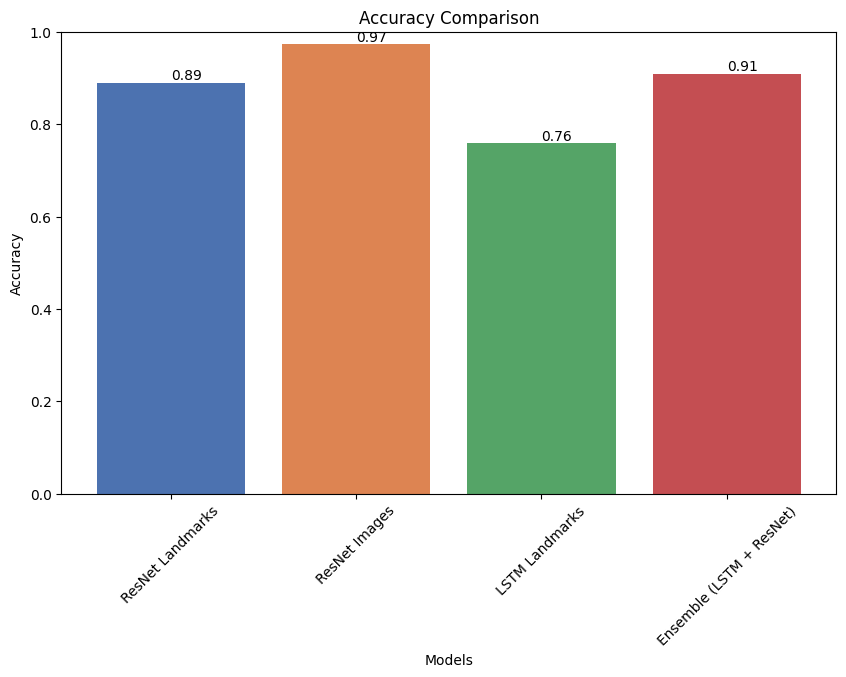
\includegraphics[width=\linewidth]{../letters-results/output.png}
\caption{ASL Alphabet test accuracy. ResNet Images leads at 0.97, followed by the ensemble at 0.91, the feed-forward MLP on landmarks at 0.89, and LSTM Landmarks at 0.76.}
\label{fig:letter-bars}
\end{figure}

Figure~\ref{fig:letter-bars} reports test accuracies for the four letter models. The ResNet on raw images comes out on top at 0.97. The feed-forward network on landmarks is second at 0.89. The ensemble (logistic regression on top of ResNet and LSTM landmark predictions) lands at 0.91. The LSTM on landmarks is the weakest at 0.76. After Bayesian tuning the landmark MLP improves to \textbf{0.9332}, which we adopt as the deployed letter model.

Why don't we deploy the 0.97 image model? The honest answer is that the Kaggle ASL Alphabet dataset has all images collected in a single session with the same signer and background. A random split puts visually similar frames in both train and test, so the test accuracy overstates how well the model would do in someone else's hand, lit differently, against a different wall. The landmark model is colder on this benchmark but only because it cannot exploit those shortcuts. In the live app (Figure~\ref{fig:app}) the landmark model is the one that survives a different signer, different lighting and a different room. We come back to this in the discussion.

\begin{figure}[t]
\centering
\begin{subfigure}{\linewidth}
  \centering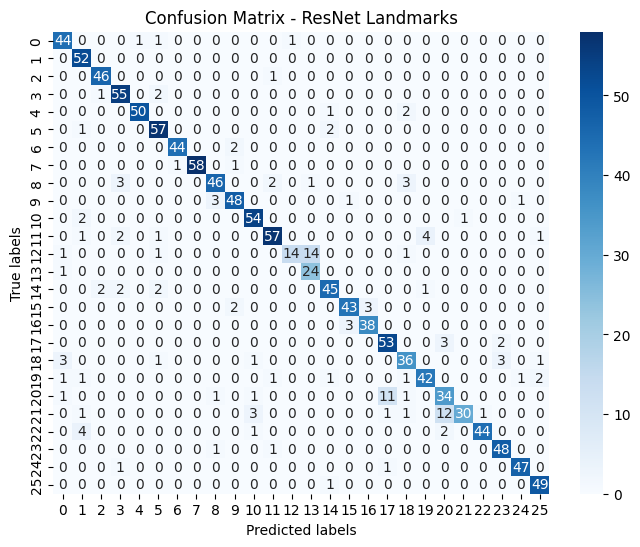
\includegraphics[width=0.95\linewidth]{../letters-results/2.png}
\end{subfigure}\\[0.4em]
\begin{subfigure}{\linewidth}
  \centering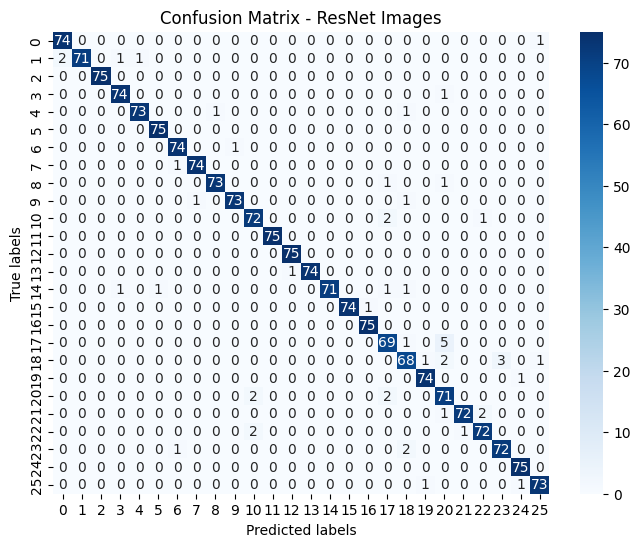
\includegraphics[width=0.95\linewidth]{../letters-results/3.png}
\end{subfigure}
\caption{Confusion matrices for the two strongest letter models. Top: the feed-forward MLP on landmarks (deployed). Bottom: ResNet on raw images. The image model has near-perfect diagonals on this benchmark; in deployment outside the original dataset it is the landmark model that holds up.}
\label{fig:letter-cm}
\end{figure}

The confusion matrices in Figure~\ref{fig:letter-cm} make the picture clearer. The image-based ResNet shows an almost perfect diagonal on the held-out test split. The landmark model also has a clean diagonal but with more off-diagonal mass on a few visually similar letter pairs (M/N, R/U). Those pairs are exactly the ones humans confuse too.

\subsection{Word Recognition}

\begin{table}[t]
\centering
\small
\begin{tabular}{lccc}
\toprule
Model & Val~T1 & Test~T1 & Test~T5 \\
\midrule
T1 WLASL-100 (75 kp) & 0.287 & 0.263 & 0.605 \\
T1 9idle-V1 (75 kp)  & 0.650 & 0.444 & 1.000 \\
T1 9idle-V2 (48 kp)  & \textbf{0.800} & \textbf{0.778} & 1.000 \\
T2 video baseline    & 0.706 & 0.429 & 1.000 \\
\bottomrule
\end{tabular}
\caption{Word-level results. Val partitions: 115, 20, 17 clips. Test partitions: 76, 13, 11 clips. Two 9-idle classes (\textit{yes} and \textit{before}) had F1 = 0 on the test split (1 and 3 samples respectively) and were soft-removed at evaluation. Training data and checkpoints are untouched.}
\label{tab:words}
\end{table}

Table~\ref{tab:words} reports validation and test top-1 / top-5 for the four word configurations. Figure~\ref{fig:val-conv} overlays the validation curves across the 120-epoch budget.

\begin{figure}[t]
\centering
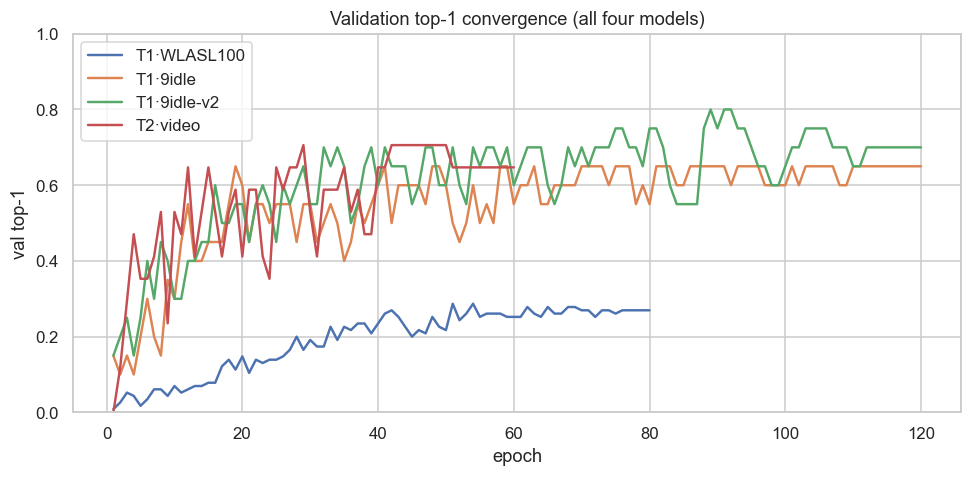
\includegraphics[width=\linewidth]{../word-results/outp5ut.png}
\caption{Validation top-1 across the 120-epoch training budget for all four word models. The pruned 48-keypoint variant (green) converges higher and faster than the full 75-keypoint version (orange).}
\label{fig:val-conv}
\end{figure}

\paragraph{Keypoint pruning helps.} The single most useful result on the word side is the V1 vs V2 comparison: dropping 27 of the 75 MediaPipe Holistic keypoints lifts validation top-1 from 65.0\% to 80.0\% on the 9-idle subset, with the same architecture, optimiser and schedule. The pruned input is also 36\% smaller and the saved model is slightly smaller on disk (3.4\,MB vs 3.6\,MB). V2 also converges faster, reaching its plateau in around 50 epochs instead of 90. We did not expect a swing of 15 absolute points from a passive choice like this.

\paragraph{Cross-track comparison.} The headline cross-track numbers were already shown in Figure~\ref{fig:cross} (Section~5.4) as a preview: when we restrict all three 9-class models to the six sign classes they can all predict --- \textit{drink, go, help, who, no, walk} --- and evaluate on the same 6-class problem, V2 wins clearly at 0.71 top-1, against 0.29 for V1 and 0.43 for the video model. A 150K-parameter Transformer on 48 keypoints beats a 123\,MB ViT-S/16 video model at this scale, which is the key practical finding behind our deployment choice.

The WLASL-100 number (28.7\% top-1) is below the strongest published baselines but matches the low end of small landmark-only models. There are two structural reasons for this. First, our model is intentionally small ($\sim$150K parameters) so that it stays on the Neural Engine. Published Pose-TGCN and graph-based baselines are 5--10 times larger. Second, WLASL-100 has roughly four training clips per class on average, and we use no large-scale pretraining. We report this number for transparency, not as a contribution.

\section{Discussion}

\paragraph{Landmarks vs images on the alphabet.} The image-based ResNet beats the landmark model on the held-out test set (0.97 vs 0.93), but we still ship the landmark model. The reason is that the Kaggle ASL Alphabet dataset is known to have within-session correlation: all images were taken in the same room with the same signer. A random split puts very similar frames into both train and test. The 0.97 number partly measures memorisation of that one session. The landmark front-end strips out the background and signer appearance and forces the model to rely on hand pose only. In the deployed app (Figure~\ref{fig:app}) it is the landmark model that holds up when a different person is signing in a different room. A cleaner benchmark with cross-signer splits would likely flip the ordering of the two models on test as well; we did not have access to one.

\paragraph{Why does keypoint pruning help so much?} Our prior was that the dropped keypoints would be uninformative. A 15-point swing is more than ``uninformative'' --- it suggests those keypoints actively hurt the model. The most likely story is that head and lower-body landmarks vary independently of the sign (the signer tilts the head, shifts weight) and feed noise into the attention layer. Removing them by hand is a cheap way to add a strong prior.

\paragraph{Why does the video model underperform?} The frozen ViT-S/16 gives strong per-frame features, but its temporal head trains from scratch on 80 clips. That is not enough data to learn the dynamics of a sign. The landmark model already has the right inductive bias built in --- its input is the motion. At a much larger data scale this ordering would likely flip. At WLASL-9 scale, it does not.

\paragraph{Why a separate idle class?} Phones are always looking. Without an idle class, the word model would emit a confident sign every frame, including when the user is doing nothing. We added \textit{idle} to the 9-idle subset for exactly this reason. It is also the class with the most training data because we pulled idle frames from the start and end of every WLASL clip.

\paragraph{Limitations.} We want to flag the obvious ones. (i) All numbers are single-seed; we did not measure variance across seeds. (ii) The WLASL test partitions are tiny --- 76, 13 and 11 clips. We rely more on validation accuracy than on test for ranking. (iii) The shipped word vocabulary is 8 signs. That is a real product constraint of the small WLASL subset we trained on, not a claim about scalability. (iv) The ASL Alphabet dataset has the within-session leakage described above, so the 0.97 image number should be read with caution. (v) We did not run a user study with deaf or hard-of-hearing participants. Any usability claims need to be qualified. (vi) The Text-to-Sign avatar fingerspells the input; it is not a learned sign synthesis model.

\paragraph{What the constraints buy us.} A few of our design choices look strange on paper. The Transformer avoids \texttt{nn.Embedding}. Input shapes are fixed. The video model takes exactly 16 frames. The landmark model takes exactly 32. These exist because the Apple Neural Engine demands them. In return the app runs at 30\,fps with the camera, the landmarks pipeline and the model all on a single phone, with no thermal throttle and no server.

\section{Conclusion}

We built a complete two-track ASL recognition and translation system that runs entirely on an iPhone. The deployed alphabet model reaches 93.32\% test accuracy on 26 letters. The deployed word model reaches 80.0\% validation top-1 on a 9-class WLASL subset with a 48-keypoint pruned skeleton. All four word models, plus the alphabet model, are exported to CoreML and run on the Apple Neural Engine. The app wraps the recognition models in a chat experience with speech-to-text, text-to-speech and a Ready Player Me avatar that can fingerspell text back, so a deaf user and a hearing partner can hold a real conversation without an interpreter.

We did not aim for state of the art on WLASL-100. We aimed for a working system. The findings we think are useful for anyone building a similar product are: (i) on a real benchmark, on-device-friendly landmark models can lose to image models that exploit dataset shortcuts, and you should test on different signers; (ii) dropping head and lower-body keypoints from MediaPipe Holistic is a free 15-point improvement on a small ASL benchmark; (iii) a 150K-parameter Transformer beats a 123\,MB frozen ViT at this data scale.

Future work includes a multi-seed re-evaluation with confidence intervals, scaling the word vocabulary toward WLASL-300, replacing the fingerspelled avatar with learned sign synthesis, and a user study with deaf and hard-of-hearing participants in real situations.

\bibliography{custom}

\end{document}
